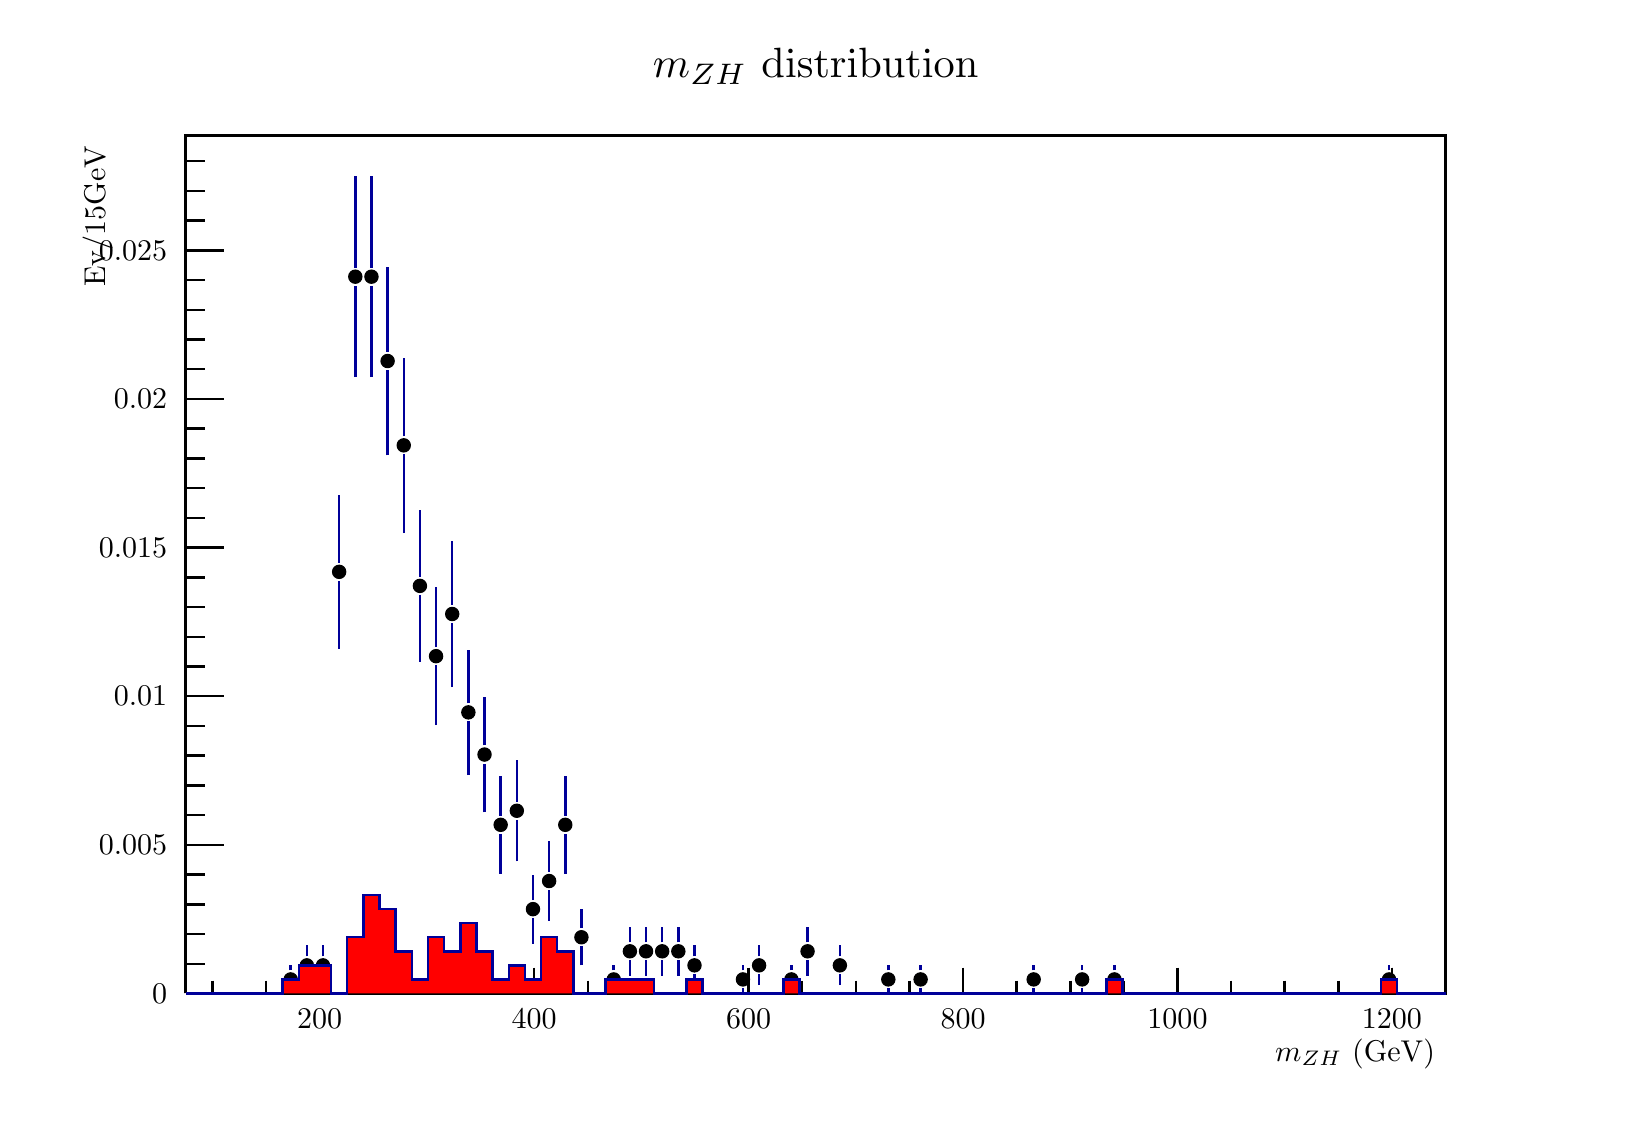
\begin{tikzpicture}
\pgfdeclareplotmark{cross} {
\pgfpathmoveto{\pgfpoint{-0.3\pgfplotmarksize}{\pgfplotmarksize}}
\pgfpathlineto{\pgfpoint{+0.3\pgfplotmarksize}{\pgfplotmarksize}}
\pgfpathlineto{\pgfpoint{+0.3\pgfplotmarksize}{0.3\pgfplotmarksize}}
\pgfpathlineto{\pgfpoint{+1\pgfplotmarksize}{0.3\pgfplotmarksize}}
\pgfpathlineto{\pgfpoint{+1\pgfplotmarksize}{-0.3\pgfplotmarksize}}
\pgfpathlineto{\pgfpoint{+0.3\pgfplotmarksize}{-0.3\pgfplotmarksize}}
\pgfpathlineto{\pgfpoint{+0.3\pgfplotmarksize}{-1.\pgfplotmarksize}}
\pgfpathlineto{\pgfpoint{-0.3\pgfplotmarksize}{-1.\pgfplotmarksize}}
\pgfpathlineto{\pgfpoint{-0.3\pgfplotmarksize}{-0.3\pgfplotmarksize}}
\pgfpathlineto{\pgfpoint{-1.\pgfplotmarksize}{-0.3\pgfplotmarksize}}
\pgfpathlineto{\pgfpoint{-1.\pgfplotmarksize}{0.3\pgfplotmarksize}}
\pgfpathlineto{\pgfpoint{-0.3\pgfplotmarksize}{0.3\pgfplotmarksize}}
\pgfpathclose
\pgfusepathqstroke
}
\pgfdeclareplotmark{cross*} {
\pgfpathmoveto{\pgfpoint{-0.3\pgfplotmarksize}{\pgfplotmarksize}}
\pgfpathlineto{\pgfpoint{+0.3\pgfplotmarksize}{\pgfplotmarksize}}
\pgfpathlineto{\pgfpoint{+0.3\pgfplotmarksize}{0.3\pgfplotmarksize}}
\pgfpathlineto{\pgfpoint{+1\pgfplotmarksize}{0.3\pgfplotmarksize}}
\pgfpathlineto{\pgfpoint{+1\pgfplotmarksize}{-0.3\pgfplotmarksize}}
\pgfpathlineto{\pgfpoint{+0.3\pgfplotmarksize}{-0.3\pgfplotmarksize}}
\pgfpathlineto{\pgfpoint{+0.3\pgfplotmarksize}{-1.\pgfplotmarksize}}
\pgfpathlineto{\pgfpoint{-0.3\pgfplotmarksize}{-1.\pgfplotmarksize}}
\pgfpathlineto{\pgfpoint{-0.3\pgfplotmarksize}{-0.3\pgfplotmarksize}}
\pgfpathlineto{\pgfpoint{-1.\pgfplotmarksize}{-0.3\pgfplotmarksize}}
\pgfpathlineto{\pgfpoint{-1.\pgfplotmarksize}{0.3\pgfplotmarksize}}
\pgfpathlineto{\pgfpoint{-0.3\pgfplotmarksize}{0.3\pgfplotmarksize}}
\pgfpathclose
\pgfusepathqfillstroke
}
\pgfdeclareplotmark{newstar} {
\pgfpathmoveto{\pgfqpoint{0pt}{\pgfplotmarksize}}
\pgfpathlineto{\pgfqpointpolar{44}{0.5\pgfplotmarksize}}
\pgfpathlineto{\pgfqpointpolar{18}{\pgfplotmarksize}}
\pgfpathlineto{\pgfqpointpolar{-20}{0.5\pgfplotmarksize}}
\pgfpathlineto{\pgfqpointpolar{-54}{\pgfplotmarksize}}
\pgfpathlineto{\pgfqpointpolar{-90}{0.5\pgfplotmarksize}}
\pgfpathlineto{\pgfqpointpolar{234}{\pgfplotmarksize}}
\pgfpathlineto{\pgfqpointpolar{198}{0.5\pgfplotmarksize}}
\pgfpathlineto{\pgfqpointpolar{162}{\pgfplotmarksize}}
\pgfpathlineto{\pgfqpointpolar{134}{0.5\pgfplotmarksize}}
\pgfpathclose
\pgfusepathqstroke
}
\pgfdeclareplotmark{newstar*} {
\pgfpathmoveto{\pgfqpoint{0pt}{\pgfplotmarksize}}
\pgfpathlineto{\pgfqpointpolar{44}{0.5\pgfplotmarksize}}
\pgfpathlineto{\pgfqpointpolar{18}{\pgfplotmarksize}}
\pgfpathlineto{\pgfqpointpolar{-20}{0.5\pgfplotmarksize}}
\pgfpathlineto{\pgfqpointpolar{-54}{\pgfplotmarksize}}
\pgfpathlineto{\pgfqpointpolar{-90}{0.5\pgfplotmarksize}}
\pgfpathlineto{\pgfqpointpolar{234}{\pgfplotmarksize}}
\pgfpathlineto{\pgfqpointpolar{198}{0.5\pgfplotmarksize}}
\pgfpathlineto{\pgfqpointpolar{162}{\pgfplotmarksize}}
\pgfpathlineto{\pgfqpointpolar{134}{0.5\pgfplotmarksize}}
\pgfpathclose
\pgfusepathqfillstroke
}
\definecolor{c}{rgb}{1,1,1};
\draw [color=c, fill=c] (0,0) rectangle (20,13.6207);
\draw [color=c, fill=c] (2,1.36207) rectangle (18,12.2586);
\definecolor{c}{rgb}{0,0,0};
\draw [c,line width=0.9] (2,1.36207) -- (2,12.2586) -- (18,12.2586) -- (18,1.36207) -- (2,1.36207);
\definecolor{c}{rgb}{1,1,1};
\draw [color=c, fill=c] (2,1.36207) rectangle (18,12.2586);
\definecolor{c}{rgb}{0,0,0};
\draw [c,line width=0.9] (2,1.36207) -- (2,12.2586) -- (18,12.2586) -- (18,1.36207) -- (2,1.36207);
\definecolor{c}{rgb}{0,0,0.6};
\draw [c,line width=0.9] (3.33333,1.36207) -- (3.33333,1.42562);
\draw [c,line width=0.9] (3.33333,1.6555) -- (3.33333,1.71905);
\definecolor{c}{rgb}{0,0,0};
\foreach \P in {(3.33333,1.54056)}{\draw[mark options={color=c,fill=c},mark size=2.402402pt,mark=*] plot coordinates {\P};}
\definecolor{c}{rgb}{0,0,0.6};
\draw [c,line width=0.9] (3.53846,1.46663) -- (3.53846,1.60411);
\draw [c,line width=0.9] (3.53846,1.83399) -- (3.53846,1.97147);
\definecolor{c}{rgb}{0,0,0};
\foreach \P in {(3.53846,1.71905)}{\draw[mark options={color=c,fill=c},mark size=2.402402pt,mark=*] plot coordinates {\P};}
\definecolor{c}{rgb}{0,0,0.6};
\draw [c,line width=0.9] (3.74359,1.46663) -- (3.74359,1.60411);
\draw [c,line width=0.9] (3.74359,1.83399) -- (3.74359,1.97147);
\definecolor{c}{rgb}{0,0,0};
\foreach \P in {(3.74359,1.71905)}{\draw[mark options={color=c,fill=c},mark size=2.402402pt,mark=*] plot coordinates {\P};}
\definecolor{c}{rgb}{0,0,0.6};
\draw [c,line width=0.9] (3.94872,5.73914) -- (3.94872,6.60183);
\draw [c,line width=0.9] (3.94872,6.83171) -- (3.94872,7.6944);
\definecolor{c}{rgb}{0,0,0};
\foreach \P in {(3.94872,6.71677)}{\draw[mark options={color=c,fill=c},mark size=2.402402pt,mark=*] plot coordinates {\P};}
\definecolor{c}{rgb}{0,0,0.6};
\draw [c,line width=0.9] (4.15385,9.19039) -- (4.15385,10.3501);
\draw [c,line width=0.9] (4.15385,10.58) -- (4.15385,11.7397);
\definecolor{c}{rgb}{0,0,0};
\foreach \P in {(4.15385,10.4651)}{\draw[mark options={color=c,fill=c},mark size=2.402402pt,mark=*] plot coordinates {\P};}
\definecolor{c}{rgb}{0,0,0.6};
\draw [c,line width=0.9] (4.35897,9.19039) -- (4.35897,10.3501);
\draw [c,line width=0.9] (4.35897,10.58) -- (4.35897,11.7397);
\definecolor{c}{rgb}{0,0,0};
\foreach \P in {(4.35897,10.4651)}{\draw[mark options={color=c,fill=c},mark size=2.402402pt,mark=*] plot coordinates {\P};}
\definecolor{c}{rgb}{0,0,0.6};
\draw [c,line width=0.9] (4.5641,8.19677) -- (4.5641,9.27918);
\draw [c,line width=0.9] (4.5641,9.50906) -- (4.5641,10.5915);
\definecolor{c}{rgb}{0,0,0};
\foreach \P in {(4.5641,9.39412)}{\draw[mark options={color=c,fill=c},mark size=2.402402pt,mark=*] plot coordinates {\P};}
\definecolor{c}{rgb}{0,0,0.6};
\draw [c,line width=0.9] (4.76923,7.20851) -- (4.76923,8.20824);
\draw [c,line width=0.9] (4.76923,8.43812) -- (4.76923,9.43785);
\definecolor{c}{rgb}{0,0,0};
\foreach \P in {(4.76923,8.32318)}{\draw[mark options={color=c,fill=c},mark size=2.402402pt,mark=*] plot coordinates {\P};}
\definecolor{c}{rgb}{0,0,0.6};
\draw [c,line width=0.9] (4.97436,5.57708) -- (4.97436,6.42334);
\draw [c,line width=0.9] (4.97436,6.65322) -- (4.97436,7.49948);
\definecolor{c}{rgb}{0,0,0};
\foreach \P in {(4.97436,6.53828)}{\draw[mark options={color=c,fill=c},mark size=2.402402pt,mark=*] plot coordinates {\P};}
\definecolor{c}{rgb}{0,0,0.6};
\draw [c,line width=0.9] (5.17949,4.77141) -- (5.17949,5.53089);
\draw [c,line width=0.9] (5.17949,5.76077) -- (5.17949,6.52025);
\definecolor{c}{rgb}{0,0,0};
\foreach \P in {(5.17949,5.64583)}{\draw[mark options={color=c,fill=c},mark size=2.402402pt,mark=*] plot coordinates {\P};}
\definecolor{c}{rgb}{0,0,0.6};
\draw [c,line width=0.9] (5.38462,5.25384) -- (5.38462,6.06636);
\draw [c,line width=0.9] (5.38462,6.29624) -- (5.38462,7.10876);
\definecolor{c}{rgb}{0,0,0};
\foreach \P in {(5.38462,6.1813)}{\draw[mark options={color=c,fill=c},mark size=2.402402pt,mark=*] plot coordinates {\P};}
\definecolor{c}{rgb}{0,0,0.6};
\draw [c,line width=0.9] (5.58974,4.13364) -- (5.58974,4.81693);
\draw [c,line width=0.9] (5.58974,5.04681) -- (5.58974,5.7301);
\definecolor{c}{rgb}{0,0,0};
\foreach \P in {(5.58974,4.93187)}{\draw[mark options={color=c,fill=c},mark size=2.402402pt,mark=*] plot coordinates {\P};}
\definecolor{c}{rgb}{0,0,0.6};
\draw [c,line width=0.9] (5.79487,3.66047) -- (5.79487,4.28146);
\draw [c,line width=0.9] (5.79487,4.51134) -- (5.79487,5.13233);
\definecolor{c}{rgb}{0,0,0};
\foreach \P in {(5.79487,4.3964)}{\draw[mark options={color=c,fill=c},mark size=2.402402pt,mark=*] plot coordinates {\P};}
\definecolor{c}{rgb}{0,0,0.6};
\draw [c,line width=0.9] (6,2.88564) -- (6,3.38901);
\draw [c,line width=0.9] (6,3.61889) -- (6,4.12226);
\definecolor{c}{rgb}{0,0,0};
\foreach \P in {(6,3.50395)}{\draw[mark options={color=c,fill=c},mark size=2.402402pt,mark=*] plot coordinates {\P};}
\definecolor{c}{rgb}{0,0,0.6};
\draw [c,line width=0.9] (6.20513,3.03888) -- (6.20513,3.5675);
\draw [c,line width=0.9] (6.20513,3.79738) -- (6.20513,4.326);
\definecolor{c}{rgb}{0,0,0};
\foreach \P in {(6.20513,3.68244)}{\draw[mark options={color=c,fill=c},mark size=2.402402pt,mark=*] plot coordinates {\P};}
\definecolor{c}{rgb}{0,0,0.6};
\draw [c,line width=0.9] (6.41026,1.9958) -- (6.41026,2.31807);
\draw [c,line width=0.9] (6.41026,2.54795) -- (6.41026,2.87022);
\definecolor{c}{rgb}{0,0,0};
\foreach \P in {(6.41026,2.43301)}{\draw[mark options={color=c,fill=c},mark size=2.402402pt,mark=*] plot coordinates {\P};}
\definecolor{c}{rgb}{0,0,0.6};
\draw [c,line width=0.9] (6.61538,2.28514) -- (6.61538,2.67505);
\draw [c,line width=0.9] (6.61538,2.90493) -- (6.61538,3.29484);
\definecolor{c}{rgb}{0,0,0};
\foreach \P in {(6.61538,2.78999)}{\draw[mark options={color=c,fill=c},mark size=2.402402pt,mark=*] plot coordinates {\P};}
\definecolor{c}{rgb}{0,0,0.6};
\draw [c,line width=0.9] (6.82051,2.88564) -- (6.82051,3.38901);
\draw [c,line width=0.9] (6.82051,3.61889) -- (6.82051,4.12226);
\definecolor{c}{rgb}{0,0,0};
\foreach \P in {(6.82051,3.50395)}{\draw[mark options={color=c,fill=c},mark size=2.402402pt,mark=*] plot coordinates {\P};}
\definecolor{c}{rgb}{0,0,0.6};
\draw [c,line width=0.9] (7.02564,1.71905) -- (7.02564,1.96109);
\draw [c,line width=0.9] (7.02564,2.19097) -- (7.02564,2.43301);
\definecolor{c}{rgb}{0,0,0};
\foreach \P in {(7.02564,2.07603)}{\draw[mark options={color=c,fill=c},mark size=2.402402pt,mark=*] plot coordinates {\P};}
\definecolor{c}{rgb}{0,0,0.6};
\draw [c,line width=0.9] (7.4359,1.36207) -- (7.4359,1.42562);
\draw [c,line width=0.9] (7.4359,1.6555) -- (7.4359,1.71905);
\definecolor{c}{rgb}{0,0,0};
\foreach \P in {(7.4359,1.54056)}{\draw[mark options={color=c,fill=c},mark size=2.402402pt,mark=*] plot coordinates {\P};}
\definecolor{c}{rgb}{0,0,0.6};
\draw [c,line width=0.9] (7.64103,1.58839) -- (7.64103,1.7826);
\draw [c,line width=0.9] (7.64103,2.01248) -- (7.64103,2.20669);
\definecolor{c}{rgb}{0,0,0};
\foreach \P in {(7.64103,1.89754)}{\draw[mark options={color=c,fill=c},mark size=2.402402pt,mark=*] plot coordinates {\P};}
\definecolor{c}{rgb}{0,0,0.6};
\draw [c,line width=0.9] (7.84615,1.58839) -- (7.84615,1.7826);
\draw [c,line width=0.9] (7.84615,2.01248) -- (7.84615,2.20669);
\definecolor{c}{rgb}{0,0,0};
\foreach \P in {(7.84615,1.89754)}{\draw[mark options={color=c,fill=c},mark size=2.402402pt,mark=*] plot coordinates {\P};}
\definecolor{c}{rgb}{0,0,0.6};
\draw [c,line width=0.9] (8.05128,1.58839) -- (8.05128,1.7826);
\draw [c,line width=0.9] (8.05128,2.01248) -- (8.05128,2.20669);
\definecolor{c}{rgb}{0,0,0};
\foreach \P in {(8.05128,1.89754)}{\draw[mark options={color=c,fill=c},mark size=2.402402pt,mark=*] plot coordinates {\P};}
\definecolor{c}{rgb}{0,0,0.6};
\draw [c,line width=0.9] (8.25641,1.58839) -- (8.25641,1.7826);
\draw [c,line width=0.9] (8.25641,2.01248) -- (8.25641,2.20669);
\definecolor{c}{rgb}{0,0,0};
\foreach \P in {(8.25641,1.89754)}{\draw[mark options={color=c,fill=c},mark size=2.402402pt,mark=*] plot coordinates {\P};}
\definecolor{c}{rgb}{0,0,0.6};
\draw [c,line width=0.9] (8.46154,1.46663) -- (8.46154,1.60411);
\draw [c,line width=0.9] (8.46154,1.83399) -- (8.46154,1.97147);
\definecolor{c}{rgb}{0,0,0};
\foreach \P in {(8.46154,1.71905)}{\draw[mark options={color=c,fill=c},mark size=2.402402pt,mark=*] plot coordinates {\P};}
\definecolor{c}{rgb}{0,0,0.6};
\draw [c,line width=0.9] (9.07692,1.36207) -- (9.07692,1.42562);
\draw [c,line width=0.9] (9.07692,1.6555) -- (9.07692,1.71905);
\definecolor{c}{rgb}{0,0,0};
\foreach \P in {(9.07692,1.54056)}{\draw[mark options={color=c,fill=c},mark size=2.402402pt,mark=*] plot coordinates {\P};}
\definecolor{c}{rgb}{0,0,0.6};
\draw [c,line width=0.9] (9.28205,1.46663) -- (9.28205,1.60411);
\draw [c,line width=0.9] (9.28205,1.83399) -- (9.28205,1.97147);
\definecolor{c}{rgb}{0,0,0};
\foreach \P in {(9.28205,1.71905)}{\draw[mark options={color=c,fill=c},mark size=2.402402pt,mark=*] plot coordinates {\P};}
\definecolor{c}{rgb}{0,0,0.6};
\draw [c,line width=0.9] (9.69231,1.36207) -- (9.69231,1.42562);
\draw [c,line width=0.9] (9.69231,1.6555) -- (9.69231,1.71905);
\definecolor{c}{rgb}{0,0,0};
\foreach \P in {(9.69231,1.54056)}{\draw[mark options={color=c,fill=c},mark size=2.402402pt,mark=*] plot coordinates {\P};}
\definecolor{c}{rgb}{0,0,0.6};
\draw [c,line width=0.9] (9.89744,1.58839) -- (9.89744,1.7826);
\draw [c,line width=0.9] (9.89744,2.01248) -- (9.89744,2.20669);
\definecolor{c}{rgb}{0,0,0};
\foreach \P in {(9.89744,1.89754)}{\draw[mark options={color=c,fill=c},mark size=2.402402pt,mark=*] plot coordinates {\P};}
\definecolor{c}{rgb}{0,0,0.6};
\draw [c,line width=0.9] (10.3077,1.46663) -- (10.3077,1.60411);
\draw [c,line width=0.9] (10.3077,1.83399) -- (10.3077,1.97147);
\definecolor{c}{rgb}{0,0,0};
\foreach \P in {(10.3077,1.71905)}{\draw[mark options={color=c,fill=c},mark size=2.402402pt,mark=*] plot coordinates {\P};}
\definecolor{c}{rgb}{0,0,0.6};
\draw [c,line width=0.9] (10.9231,1.36207) -- (10.9231,1.42562);
\draw [c,line width=0.9] (10.9231,1.6555) -- (10.9231,1.71905);
\definecolor{c}{rgb}{0,0,0};
\foreach \P in {(10.9231,1.54056)}{\draw[mark options={color=c,fill=c},mark size=2.402402pt,mark=*] plot coordinates {\P};}
\definecolor{c}{rgb}{0,0,0.6};
\draw [c,line width=0.9] (11.3333,1.36207) -- (11.3333,1.42562);
\draw [c,line width=0.9] (11.3333,1.6555) -- (11.3333,1.71905);
\definecolor{c}{rgb}{0,0,0};
\foreach \P in {(11.3333,1.54056)}{\draw[mark options={color=c,fill=c},mark size=2.402402pt,mark=*] plot coordinates {\P};}
\definecolor{c}{rgb}{0,0,0.6};
\draw [c,line width=0.9] (12.7692,1.36207) -- (12.7692,1.42562);
\draw [c,line width=0.9] (12.7692,1.6555) -- (12.7692,1.71905);
\definecolor{c}{rgb}{0,0,0};
\foreach \P in {(12.7692,1.54056)}{\draw[mark options={color=c,fill=c},mark size=2.402402pt,mark=*] plot coordinates {\P};}
\definecolor{c}{rgb}{0,0,0.6};
\draw [c,line width=0.9] (13.3846,1.36207) -- (13.3846,1.42562);
\draw [c,line width=0.9] (13.3846,1.6555) -- (13.3846,1.71905);
\definecolor{c}{rgb}{0,0,0};
\foreach \P in {(13.3846,1.54056)}{\draw[mark options={color=c,fill=c},mark size=2.402402pt,mark=*] plot coordinates {\P};}
\definecolor{c}{rgb}{0,0,0.6};
\draw [c,line width=0.9] (13.7949,1.36207) -- (13.7949,1.42562);
\draw [c,line width=0.9] (13.7949,1.6555) -- (13.7949,1.71905);
\definecolor{c}{rgb}{0,0,0};
\foreach \P in {(13.7949,1.54056)}{\draw[mark options={color=c,fill=c},mark size=2.402402pt,mark=*] plot coordinates {\P};}
\definecolor{c}{rgb}{0,0,0.6};
\draw [c,line width=0.9] (17.2821,1.36207) -- (17.2821,1.42562);
\draw [c,line width=0.9] (17.2821,1.6555) -- (17.2821,1.71905);
\definecolor{c}{rgb}{0,0,0};
\foreach \P in {(17.2821,1.54056)}{\draw[mark options={color=c,fill=c},mark size=2.402402pt,mark=*] plot coordinates {\P};}
\draw [c,line width=0.9] (2,1.36207) -- (18,1.36207);
\draw [anchor= east] (18,0.599311) node[scale=1.08496, color=c, rotate=0]{$m_{ZH} \mbox{ (GeV)}$};
\draw [c,line width=0.9] (3.70213,1.68897) -- (3.70213,1.36207);
\draw [c,line width=0.9] (4.38298,1.52552) -- (4.38298,1.36207);
\draw [c,line width=0.9] (5.06383,1.52552) -- (5.06383,1.36207);
\draw [c,line width=0.9] (5.74468,1.52552) -- (5.74468,1.36207);
\draw [c,line width=0.9] (6.42553,1.68897) -- (6.42553,1.36207);
\draw [c,line width=0.9] (7.10638,1.52552) -- (7.10638,1.36207);
\draw [c,line width=0.9] (7.78723,1.52552) -- (7.78723,1.36207);
\draw [c,line width=0.9] (8.46809,1.52552) -- (8.46809,1.36207);
\draw [c,line width=0.9] (9.14894,1.68897) -- (9.14894,1.36207);
\draw [c,line width=0.9] (9.82979,1.52552) -- (9.82979,1.36207);
\draw [c,line width=0.9] (10.5106,1.52552) -- (10.5106,1.36207);
\draw [c,line width=0.9] (11.1915,1.52552) -- (11.1915,1.36207);
\draw [c,line width=0.9] (11.8723,1.68897) -- (11.8723,1.36207);
\draw [c,line width=0.9] (12.5532,1.52552) -- (12.5532,1.36207);
\draw [c,line width=0.9] (13.234,1.52552) -- (13.234,1.36207);
\draw [c,line width=0.9] (13.9149,1.52552) -- (13.9149,1.36207);
\draw [c,line width=0.9] (14.5957,1.68897) -- (14.5957,1.36207);
\draw [c,line width=0.9] (15.2766,1.52552) -- (15.2766,1.36207);
\draw [c,line width=0.9] (15.9574,1.52552) -- (15.9574,1.36207);
\draw [c,line width=0.9] (16.6383,1.52552) -- (16.6383,1.36207);
\draw [c,line width=0.9] (17.3191,1.68897) -- (17.3191,1.36207);
\draw [c,line width=0.9] (3.70213,1.68897) -- (3.70213,1.36207);
\draw [c,line width=0.9] (3.02128,1.52552) -- (3.02128,1.36207);
\draw [c,line width=0.9] (2.34043,1.52552) -- (2.34043,1.36207);
\draw [c,line width=0.9] (17.3191,1.68897) -- (17.3191,1.36207);
\draw [c,line width=0.9] (18,1.52552) -- (18,1.36207);
\draw [anchor=base] (3.70213,0.912586) node[scale=1.08496, color=c, rotate=0]{200};
\draw [anchor=base] (6.42553,0.912586) node[scale=1.08496, color=c, rotate=0]{400};
\draw [anchor=base] (9.14894,0.912586) node[scale=1.08496, color=c, rotate=0]{600};
\draw [anchor=base] (11.8723,0.912586) node[scale=1.08496, color=c, rotate=0]{800};
\draw [anchor=base] (14.5957,0.912586) node[scale=1.08496, color=c, rotate=0]{1000};
\draw [anchor=base] (17.3191,0.912586) node[scale=1.08496, color=c, rotate=0]{1200};
\draw [c,line width=0.9] (2,1.36207) -- (2,12.2586);
\draw [anchor= east] (0.88,12.2586) node[scale=1.08496, color=c, rotate=90]{$\mbox{Ev/15GeV}$};
\draw [c,line width=0.9] (2.48,1.36207) -- (2,1.36207);
\draw [c,line width=0.9] (2.24,1.73958) -- (2,1.73958);
\draw [c,line width=0.9] (2.24,2.11708) -- (2,2.11708);
\draw [c,line width=0.9] (2.24,2.49459) -- (2,2.49459);
\draw [c,line width=0.9] (2.24,2.8721) -- (2,2.8721);
\draw [c,line width=0.9] (2.48,3.2496) -- (2,3.2496);
\draw [c,line width=0.9] (2.24,3.62711) -- (2,3.62711);
\draw [c,line width=0.9] (2.24,4.00461) -- (2,4.00461);
\draw [c,line width=0.9] (2.24,4.38212) -- (2,4.38212);
\draw [c,line width=0.9] (2.24,4.75963) -- (2,4.75963);
\draw [c,line width=0.9] (2.48,5.13713) -- (2,5.13713);
\draw [c,line width=0.9] (2.24,5.51464) -- (2,5.51464);
\draw [c,line width=0.9] (2.24,5.89215) -- (2,5.89215);
\draw [c,line width=0.9] (2.24,6.26965) -- (2,6.26965);
\draw [c,line width=0.9] (2.24,6.64716) -- (2,6.64716);
\draw [c,line width=0.9] (2.48,7.02467) -- (2,7.02467);
\draw [c,line width=0.9] (2.24,7.40217) -- (2,7.40217);
\draw [c,line width=0.9] (2.24,7.77968) -- (2,7.77968);
\draw [c,line width=0.9] (2.24,8.15719) -- (2,8.15719);
\draw [c,line width=0.9] (2.24,8.53469) -- (2,8.53469);
\draw [c,line width=0.9] (2.48,8.9122) -- (2,8.9122);
\draw [c,line width=0.9] (2.24,9.28971) -- (2,9.28971);
\draw [c,line width=0.9] (2.24,9.66721) -- (2,9.66721);
\draw [c,line width=0.9] (2.24,10.0447) -- (2,10.0447);
\draw [c,line width=0.9] (2.24,10.4222) -- (2,10.4222);
\draw [c,line width=0.9] (2.48,10.7997) -- (2,10.7997);
\draw [c,line width=0.9] (2.48,10.7997) -- (2,10.7997);
\draw [c,line width=0.9] (2.24,11.1772) -- (2,11.1772);
\draw [c,line width=0.9] (2.24,11.5547) -- (2,11.5547);
\draw [c,line width=0.9] (2.24,11.9323) -- (2,11.9323);
\draw [anchor= east] (1.9,1.36207) node[scale=1.08496, color=c, rotate=0]{0};
\draw [anchor= east] (1.9,3.2496) node[scale=1.08496, color=c, rotate=0]{0.005};
\draw [anchor= east] (1.9,5.13713) node[scale=1.08496, color=c, rotate=0]{0.01};
\draw [anchor= east] (1.9,7.02467) node[scale=1.08496, color=c, rotate=0]{0.015};
\draw [anchor= east] (1.9,8.9122) node[scale=1.08496, color=c, rotate=0]{0.02};
\draw [anchor= east] (1.9,10.7997) node[scale=1.08496, color=c, rotate=0]{0.025};
\definecolor{c}{rgb}{1,0,0};
\draw [c, fill=c] (2,1.36207) -- (2,1.36207) -- (2.20513,1.36207) -- (2.20513,1.36207) -- (2.41026,1.36207) -- (2.41026,1.36207) -- (2.61538,1.36207) -- (2.61538,1.36207) -- (2.82051,1.36207) -- (2.82051,1.36207) -- (3.02564,1.36207) --
 (3.02564,1.36207) -- (3.23077,1.36207) -- (3.23077,1.54056) -- (3.4359,1.54056) -- (3.4359,1.71905) -- (3.64103,1.71905) -- (3.64103,1.71905) -- (3.84615,1.71905) -- (3.84615,1.36207) -- (4.05128,1.36207) -- (4.05128,2.07603) -- (4.25641,2.07603) --
 (4.25641,2.6115) -- (4.46154,2.6115) -- (4.46154,2.43301) -- (4.66667,2.43301) -- (4.66667,1.89754) -- (4.8718,1.89754) -- (4.8718,1.54056) -- (5.07692,1.54056) -- (5.07692,2.07603) -- (5.28205,2.07603) -- (5.28205,1.89754) -- (5.48718,1.89754) --
 (5.48718,2.25452) -- (5.69231,2.25452) -- (5.69231,1.89754) -- (5.89744,1.89754) -- (5.89744,1.54056) -- (6.10256,1.54056) -- (6.10256,1.71905) -- (6.30769,1.71905) -- (6.30769,1.54056) -- (6.51282,1.54056) -- (6.51282,2.07603) -- (6.71795,2.07603)
 -- (6.71795,1.89754) -- (6.92308,1.89754) -- (6.92308,1.36207) -- (7.12821,1.36207) -- (7.12821,1.36207) -- (7.33333,1.36207) -- (7.33333,1.54056) -- (7.53846,1.54056) -- (7.53846,1.54056) -- (7.74359,1.54056) -- (7.74359,1.54056) --
 (7.94872,1.54056) -- (7.94872,1.36207) -- (8.15385,1.36207) -- (8.15385,1.36207) -- (8.35897,1.36207) -- (8.35897,1.54056) -- (8.5641,1.54056) -- (8.5641,1.36207) -- (8.76923,1.36207) -- (8.76923,1.36207) -- (8.97436,1.36207) -- (8.97436,1.36207) --
 (9.17949,1.36207) -- (9.17949,1.36207) -- (9.38461,1.36207) -- (9.38461,1.36207) -- (9.58974,1.36207) -- (9.58974,1.54056) -- (9.79487,1.54056) -- (9.79487,1.36207) -- (10,1.36207) -- (10,1.36207) -- (10.2051,1.36207) -- (10.2051,1.36207) --
 (10.4103,1.36207) -- (10.4103,1.36207) -- (10.6154,1.36207) -- (10.6154,1.36207) -- (10.8205,1.36207) -- (10.8205,1.36207) -- (11.0256,1.36207) -- (11.0256,1.36207) -- (11.2308,1.36207) -- (11.2308,1.36207) -- (11.4359,1.36207) -- (11.4359,1.36207)
 -- (11.641,1.36207) -- (11.641,1.36207) -- (11.8462,1.36207) -- (11.8462,1.36207) -- (12.0513,1.36207) -- (12.0513,1.36207) -- (12.2564,1.36207) -- (12.2564,1.36207) -- (12.4615,1.36207) -- (12.4615,1.36207) -- (12.6667,1.36207) -- (12.6667,1.36207)
 -- (12.8718,1.36207) -- (12.8718,1.36207) -- (13.0769,1.36207) -- (13.0769,1.36207) -- (13.2821,1.36207) -- (13.2821,1.36207) -- (13.4872,1.36207) -- (13.4872,1.36207) -- (13.6923,1.36207) -- (13.6923,1.54056) -- (13.8974,1.54056) --
 (13.8974,1.36207) -- (14.1026,1.36207) -- (14.1026,1.36207) -- (14.3077,1.36207) -- (14.3077,1.36207) -- (14.5128,1.36207) -- (14.5128,1.36207) -- (14.7179,1.36207) -- (14.7179,1.36207) -- (14.9231,1.36207) -- (14.9231,1.36207) -- (15.1282,1.36207)
 -- (15.1282,1.36207) -- (15.3333,1.36207) -- (15.3333,1.36207) -- (15.5385,1.36207) -- (15.5385,1.36207) -- (15.7436,1.36207) -- (15.7436,1.36207) -- (15.9487,1.36207) -- (15.9487,1.36207) -- (16.1538,1.36207) -- (16.1538,1.36207) --
 (16.359,1.36207) -- (16.359,1.36207) -- (16.5641,1.36207) -- (16.5641,1.36207) -- (16.7692,1.36207) -- (16.7692,1.36207) -- (16.9744,1.36207) -- (16.9744,1.36207) -- (17.1795,1.36207) -- (17.1795,1.54056) -- (17.3846,1.54056) -- (17.3846,1.36207) --
 (17.5897,1.36207) -- (17.5897,1.36207) -- (17.7949,1.36207) -- (17.7949,1.36207) -- (18,1.36207) -- (18,1.36207);
\definecolor{c}{rgb}{0,0,0.6};
\draw [c,line width=0.9] (2,1.36207) -- (2.20513,1.36207) -- (2.20513,1.36207) -- (2.41026,1.36207) -- (2.41026,1.36207) -- (2.61538,1.36207) -- (2.61538,1.36207) -- (2.82051,1.36207) -- (2.82051,1.36207) -- (3.02564,1.36207) -- (3.02564,1.36207) --
 (3.23077,1.36207) -- (3.23077,1.54056) -- (3.4359,1.54056) -- (3.4359,1.71905) -- (3.64103,1.71905) -- (3.64103,1.71905) -- (3.84615,1.71905) -- (3.84615,1.36207) -- (4.05128,1.36207) -- (4.05128,2.07603) -- (4.25641,2.07603) -- (4.25641,2.6115) --
 (4.46154,2.6115) -- (4.46154,2.43301) -- (4.66667,2.43301) -- (4.66667,1.89754) -- (4.8718,1.89754) -- (4.8718,1.54056) -- (5.07692,1.54056) -- (5.07692,2.07603) -- (5.28205,2.07603) -- (5.28205,1.89754) -- (5.48718,1.89754) -- (5.48718,2.25452) --
 (5.69231,2.25452) -- (5.69231,1.89754) -- (5.89744,1.89754) -- (5.89744,1.54056) -- (6.10256,1.54056) -- (6.10256,1.71905) -- (6.30769,1.71905) -- (6.30769,1.54056) -- (6.51282,1.54056) -- (6.51282,2.07603) -- (6.71795,2.07603) -- (6.71795,1.89754)
 -- (6.92308,1.89754) -- (6.92308,1.36207) -- (7.12821,1.36207) -- (7.12821,1.36207) -- (7.33333,1.36207) -- (7.33333,1.54056) -- (7.53846,1.54056) -- (7.53846,1.54056) -- (7.74359,1.54056) -- (7.74359,1.54056) -- (7.94872,1.54056) --
 (7.94872,1.36207) -- (8.15385,1.36207) -- (8.15385,1.36207) -- (8.35897,1.36207) -- (8.35897,1.54056) -- (8.5641,1.54056) -- (8.5641,1.36207) -- (8.76923,1.36207) -- (8.76923,1.36207) -- (8.97436,1.36207) -- (8.97436,1.36207) -- (9.17949,1.36207) --
 (9.17949,1.36207) -- (9.38461,1.36207) -- (9.38461,1.36207) -- (9.58974,1.36207) -- (9.58974,1.54056) -- (9.79487,1.54056) -- (9.79487,1.36207) -- (10,1.36207) -- (10,1.36207) -- (10.2051,1.36207) -- (10.2051,1.36207) -- (10.4103,1.36207) --
 (10.4103,1.36207) -- (10.6154,1.36207) -- (10.6154,1.36207) -- (10.8205,1.36207) -- (10.8205,1.36207) -- (11.0256,1.36207) -- (11.0256,1.36207) -- (11.2308,1.36207) -- (11.2308,1.36207) -- (11.4359,1.36207) -- (11.4359,1.36207) -- (11.641,1.36207)
 -- (11.641,1.36207) -- (11.8462,1.36207) -- (11.8462,1.36207) -- (12.0513,1.36207) -- (12.0513,1.36207) -- (12.2564,1.36207) -- (12.2564,1.36207) -- (12.4615,1.36207) -- (12.4615,1.36207) -- (12.6667,1.36207) -- (12.6667,1.36207) --
 (12.8718,1.36207) -- (12.8718,1.36207) -- (13.0769,1.36207) -- (13.0769,1.36207) -- (13.2821,1.36207) -- (13.2821,1.36207) -- (13.4872,1.36207) -- (13.4872,1.36207) -- (13.6923,1.36207) -- (13.6923,1.54056) -- (13.8974,1.54056) -- (13.8974,1.36207)
 -- (14.1026,1.36207) -- (14.1026,1.36207) -- (14.3077,1.36207) -- (14.3077,1.36207) -- (14.5128,1.36207) -- (14.5128,1.36207) -- (14.7179,1.36207) -- (14.7179,1.36207) -- (14.9231,1.36207) -- (14.9231,1.36207) -- (15.1282,1.36207) --
 (15.1282,1.36207) -- (15.3333,1.36207) -- (15.3333,1.36207) -- (15.5385,1.36207) -- (15.5385,1.36207) -- (15.7436,1.36207) -- (15.7436,1.36207) -- (15.9487,1.36207) -- (15.9487,1.36207) -- (16.1538,1.36207) -- (16.1538,1.36207) -- (16.359,1.36207)
 -- (16.359,1.36207) -- (16.5641,1.36207) -- (16.5641,1.36207) -- (16.7692,1.36207) -- (16.7692,1.36207) -- (16.9744,1.36207) -- (16.9744,1.36207) -- (17.1795,1.36207) -- (17.1795,1.54056) -- (17.3846,1.54056) -- (17.3846,1.36207) --
 (17.5897,1.36207) -- (17.5897,1.36207) -- (17.7949,1.36207) -- (17.7949,1.36207) -- (18,1.36207);
\definecolor{c}{rgb}{0,0,0};
\draw (10,13.1388) node[scale=1.5317, color=c, rotate=0]{$m_{ZH} \mbox{ distribution}$};
\end{tikzpicture}
